\begin{tikzpicture}[scale=1.1]
\draw[MidnightBlue!40] (0,0) circle (1.1);
\draw[->,MidnightBlue,thick] (0,0)--(1.1,0) node[right] {$1$};
\draw[->,MidnightBlue,thick] (0,0)--(38:1.1) node[above right] {$q$};
\draw[->,MidnightBlue,thick] (0,0)--(76:1.1) node[above] {$q^2$};
\draw[->,BurntOrange,thick] (0,0)--(114:1.1) node[above left] {$q^3$};
\node[align=center] at (4,0.45) {$1+q+\cdots+q^{N-1}=\dfrac{1-q^N}{1-q}$};
\node at (4,-.55) {$q=e(k\alpha)\ne1$};
\node at (3,-1.5) {$\left|N^{-1}\sum_{j<N}q^j\right|\le \dfrac{2}{N|1-q|}$};
\end{tikzpicture}
